\documentclass[a4paper,12pt]{article}

\usepackage[1925275]{MCMthesis}\problem{D}
\usepackage{palatino}
\usepackage{natbib}
\usepackage{graphicx}
\usepackage{minted}
\usepackage{float}
\usepackage{appendix}
\usepackage{threeparttable}
\usepackage{supertabular}
\usepackage{url}
\usepackage{amsmath}
\usepackage{textcomp,booktabs}
\usepackage[usenames,dvipsnames]{color}
\usepackage{colortbl}
\definecolor{mygray}{gray}{.9}
\definecolor{mypink}{rgb}{.99,.91,.95}
\definecolor{mycyan}{cmyk}{.3,0,0,0}


\setlength{\belowcaptionskip}{4pt}
\setlength{\abovecaptionskip}{4pt}

\usepackage{titlesec}
\usepackage{titletoc}
\setcounter{tocdepth}{2}



\titlecontents{section}[12mm]{\fontsize{12pt}{32pt}\selectfont \bf}{\contentslabel{2.5em}}{}{\titlerule*{.}\contentspage}
\titlecontents{subsection}[18mm]{\fontsize{12pt}{22pt}\selectfont \fs}{\contentslabel{3.3em}}{}{\titlerule*{.}\contentspage}

\usepackage[font=small,]{caption}
\title{GUSH Model for Emergency Evacuation Planning}  %Title

\begin{document}



%----------Summary----------
\begin{abstract}\footnotesize 
The evacuation problem of public places is of great concern around the world. Facing the threat of terror attacks, the Louvre needs to design an evacuation plan that's effective and efficient.  

Now there are mainly two ways to make the evacuation planning: \textbf{network flow models}, assuming everyone is under control; and \textbf{probability models}, focusing on individual behavior. In this paper, we combine these two approaches and present a novel \textbf{GUSH (Global gUidance - perSonal beHavior) model}. Global guidance means that the managers give real-time and dynamic guidance for everyone, which is an optimal plan for all the people as a whole. It is realized by an \textbf{App} serving as a guide during the evacuation. Meanwhile, this model also considers personal psychology and behavior that affect the ideal plan given by the managers. 

Firstly, we adopt the \textbf{dynamic maximal flow model} as the basic model to build the GUSH model. The dynamic maximal flow model can find out a plan consuming the shortest time for the whole people. We draw the network graph of the Louvre and use the \textbf{Edmond-Karp algorithm} to calculate the model. The optimal routes for everyone are shown and the shortest evacuation time is 11.6 minutes.

Secondly, we introduce the \textbf{selfishness factor} into the basic model to describe the effect of the selfish people. It is based on the judgement that people who are selfish tend to take the shortest way and deviate from the way allocated to them. In addition, to design the best route for the disabled people, we introduce the \textbf{disabled people factor}. We assume the disabled exclude the passages with high popularity density and \textbf{take the shortest way} to the elevators specially prepared for them. What's more, we introduce an \textbf{emergency personnel factor} to design the route for the emergency personnel entering the museum. They take the shortest way to the bottlenecks to manage the crowd. By applying this adjusted GUSH model to the Louvre, we find the \textbf{bottlenecks} that should be paid attention to if the owner wants to shorten the evacuation time.

Thirdly, we create an example to justify our model. Assuming a terror attack happens in the museum at a random place on a random day, we use our model to formulate the most effective evacuation plan and calculate the total time. From this example, it's clear that our model is able to address various types of potential threats. We also conduct \textbf{sensitivity analysis} on the flow speed and the capacity of bottlenecks. It proves that the evacuation time takes on the shape of \textbf{ "U" } with the increasing of the flow speed. Meanwhile, the speed at which the evacuation time gets shorter slows down with the expansion of the bottlenecks. According to these results, we propose suggestions to the museum owners.  

Finally, we discuss the strengths and weaknesses of the proposed models. It's believed that our model is adaptable. It can be adopted to help design the evacuation plan for other large, crowded structures.





\end{abstract}

\maketitle
\thispagestyle{empty}

\newpage
\setcounter{tocdepth}{3}
\tableofcontents
\thispagestyle{empty}
\newpage

\setlength\parskip{0.8\baselineskip}
\setcounter{page}{1}
\pagestyle{fancy}

\section{Introduction}
\subsection{Background}

The emergency evacuation is one of the most important issues a popular destination must pay attention to, especially in these days when terror attacks happen from time to time. In Paris, the Louvre welcomes millions of visitors every year, home and abroad. Nothing can compromise the critical role of a reasonable evacuation plan in case anything urgent takes place in the museum. 


\subsection{Problem Statement and Analysis}

To formulate an evacuation plan, it's straightforward that the \textbf{goal} is to determine an evacuation routing that allows all the occupants leave the building as quickly and securely as possible. 

Interested in this problem, several methods have been adopted to address it, among which the \textbf{network models} are the most popular. For example, someone transforms the problem into a \textbf{minimal cost flow problem} on a slighted modified graph \citep{TAKEOYAMADA1996A}, while some others solve this problem using the dynamic network model with the procedure of \textbf{Edmond-Karp algorithm} \citep{edmonds1972theoretical}.

The shortcomings of the network model is that it doesn't consider the behavior of individuals. To solve this problem, somebody builds a \textbf{probabilistic model} and develops a \textbf{divide-and-conquer approach} \citep{Wang2008Modeling}. However, this way is focused on each person and loses a "global view". These two models are complementary \citep{Chalmet1982Network}, and there's a need to combine these two approaches. Based on it, we establish a \textbf{GUSH (Global gUidance - perSonal beHavior) model}. 

\subsection{Our work}
To further present our solutions, we arrange our paper as follows.
\begin{itemize}
\item \textbf{In section 2}, we give out the reliable assumptions to simplify the model.
\item \textbf{In section 3}, we introduce the methodology. We first construct a dynamic maximal flow model. Based on it we build a GUSH model, taking human behavior factors into consideration. We also adjust the GUSH model by including other factors such as the disabled people and the emergency personnel.
\item \textbf{In section 4}, we apply our model to determine an optimal evacuation plan for the Louvre. We consider several factors to make our model more adaptable to the real situation. A specific example is given to show how our model works facing a specific urgency.
\item \textbf{In section 5}, we carry out sensitivity analysis of the flow speed and the capacity of bottlenecks.
\item \textbf{At last}, we discuss the strengths and weaknesses of our model in detail and make conclusions. We give suggestions to the emergency management department of the Louvre.
\end{itemize}

\section{Assumptions}
\begin{itemize}
\item By technology, the emergency personnel of the Louvre can locate everyone instantly. Using a certain model, it can provide the optimal route for everyone dynamically. 
\item The Louvre can provide the evacuation guide function in its official App. It serves as a 
navigation, instructing the best way when emergency happens. Most people install the app and follow the instruction of the app, while some people who are selfish don't follow it, but tend to choose the shortest way out.
\item We assume that the capacity of the components of a building (rooms, stairs, passages, etc.) is proportional to their space area, which can be estimated from the map provided on the official website of Louvre (\url{https://www.louvre.fr/en/plan}). To make it simpler, we assume each stair has the same capacity.
\item We don't consider elevators since we assume the emergency (such as fire or bombing) will make it unsafe to take the elevator, but We assume there are elevators specially for the disabled when emergency happens.
\item Since the entrances/exits are blocked because of the outflow of people, the emergency personnel all enter through the extra entrances on the ground floor. They are commanded by the app and move to the most crowded places to help control the crowd. Because we don't know the location of the extra entrances, we assume the extra entrances distribute uniformly in the Louvre. To simplify the model, we assume the emergency personnel are only responsible for crowd control.
\end{itemize}

\section{Glossary \& Symbols} 
\subsection{Glossary}
\paragraph{Being selfish} If everyone follows the App, the overall time is shortest, but some people may take a detour and be the last to evacuate. Ideally, everyone follows the instruction. However, considering the selfishness of human nature, people tend to make decisions in their own interests. We think a man who is “selfish” tends to take the shortest route, rather than the guided route.
\paragraph{Selfishness factor}  Some people may not follow the guide but take the shortest way to the nearest exit out of selfishness. Consequently, they deviate from the appointed route and disturb the global optimal model result, making the total evacuation time longer. The degree to which those selfish people affect the overall optimal model is defined as the "selfishness factor".
\paragraph{Disabled people factor} The disabled have special needs that make their optimal routing different from normal people. We define the degree to which those disabled people affect the GUSH model as the "disabled people factor".
\paragraph{Emergency personnel factor} The emergency personnel enter the building. They head to the most crowded passages to help control the crowd. We define the degree to which the emergency personnel affect the GUSH model as the "emergency personnel factor".
\subsection{Symbols}

\begin{center}
\topcaption{Symbols\label{tab1}}
%
\tablefirsthead{\toprule\multicolumn{1}{c}{\textbf{Symbol}}&\multicolumn{1}{c}{\textbf{Definition}}\\\midrule}
\tablelasttail{\bottomrule}
%
\tablehead{\midrule}
\tabletail{\midrule}

\begin{supertabular}{p{2cm}<{\centering}p{10cm}<{\centering}}
 $v_s$ & the source node \\ 
 $v_e$ & the sink node \\
 $v_i$ & the node $i$\\
 $v_iv_j$ & the edge connecting $v_i$ and $v_j$\\
 $\bm{E}$ & the set of the edges\\
 $C_{ij}$ & the capacity of the edge $v_iv_j$\\
 $f_{ij}$ & the flow of the edge $v_iv_j$\\
 $C^t_{ij}$ & the capacity of the edge $v_iv_j$ in the time period $t$\\ 
 $f^t_{ij}$ & the flow of the edge $v_iv_j$ in the time period $t$\\
 x & each person in the building\\
 $\bm{M}$ & the set of all the persons in the building\\
 $\bm{S}$ & the set of all the selfish persons in the building\\
 $\bm{D}$ & the set of all the disabled persons in the building\\
 $t$ & the time period of the dynamic optimal flow model \\
 $n$& the total number of the time periods\\
 $p^t_x$ & the possibility of the person x being selfish in the time period t\\
\end{supertabular}
\end{center}




\section{Model for Evacuation Planning}
In this section we develop three models: the dynamic maximal flow model, the GUSH model and the adjusted GUSH model. The last two are both established based on the first basic.
\subsection{Global Guidance: Dynamic Maximal Flow Model} 
The maximal flow model is effective to figure out the overall quickest evacuation routing in a building \citep{lim2012capacitated}. Since the emergency personnel have the instant location of people, they can use this model and adjust the guide frequently, depending on the constant change of the distribution of people.

To use this model, firstly, we need to draw the network graph . As is shown in Figure \ref{fig4-1}, we see each component as a node and each passage as an edge. We add a source node and connect it to the node of each room. The capacity of these edges is the number of people in this room. We also add a sink node and connect it to the exits. The capacity of these edges is infinite. The capacity of other edges is the capacity of passages.

\begin{figure} [H]
\centering
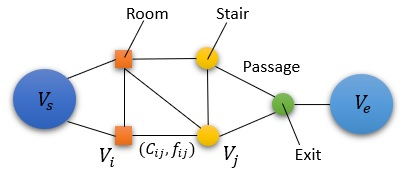
\includegraphics{networkflow.jpg}
\caption{Network Graph}
\label{fig4-1}
\end{figure}

This maximal flow model should be dynamic. For each of the period $t$, the capacity of edges changes because some people already flow out. We consider the following.
\begin{eqnarray}
\label{equ1}
 & \textrm{maximize} &               \ \    \sum \limits_{(v_i,v_j)\in \bm{E}} f^t_{ij},\quad t=1, 2, \ldots,n \nonumber \\
 & \textrm{subject}\ \textrm{to} &    \ \   0\leq f^t_{ij}\leq C^t_{ij}\\
 &   &  \ \ 
\sum_{(v_i,v_k) \in  \bm{E}}f^t_{ik} - \sum_{(v_j,v_i)\in  \bm{E}}f^t_{ji}= 
\left\{\begin{matrix}
\sum\limits_{(v_i,v_j) \in  \bm{E}}f^t_{ij} & i=s\\ 
0 & i \neq s,e\\ 
-\sum\limits_{(v_i,v_j) \in  \bm{E}}f^t_{ij} & i=e
\end{matrix}\right. \nonumber
\end{eqnarray}
where $v_i$ denotes the node $i$,  $f^t_{ij}$ and $C^t_{ij}$ respectively represents the flow and the capacity of the edge $v_iv_j$ in the time period $t$.

\subsection{Personal Behavior: GUSH Model}
Personal behavior is a significant factor when making the evacuation plan. Faced with urgent situations, people probably become panic, fear, and as a result, out of control \citep{zhang2005personal}. Here in our basic model, since people can see the nearest exit in the App,  they may also be uncontrollable out of selfishness. Although the basic model is the most timesaving plan for all, some people may take a detour and be the last to evacuate. For these people, chances are that they may choose the shortest way in their own interests. To take this into consideration, we add a selfishness factor to the basic model:

\begin{equation}
\label{equ2}
C^t_{ij}=C^{t-1}_{ij}-s^{t-1}_{ij},\ \ t = 2,3,\ldots, n
\end{equation}
  where $C^1_{ij}$ denotes the initial capacity of the edge $v_iv_j$.

It means in each time period $t$, the capacity of the edge $v_iv_j$ should be the capacity of the last period deducting the selfishness factor. This is because those selfish people occupy the passages which are not allocated to them, making this passage more crowded and prevent some others from passing through this way.

We use the \textbf{Dijkstra Algorithm} to formulate the shortest route. For each person x, defining $\bm{B}_x$ as the set of edges of the shortest route the selfish person x takes, $\bm{A}_x$ as the set of edges of the guided route the selfish person x should take initially, we have

\begin{equation}
\label{equ3}
a^{t}_{xij}=\left\{\begin{matrix}
1 &v_iv_j\in \bm{B}^t_x \\ 
-1 & v_iv_j\in \bm{A}^t_x\\
0 & else
\end{matrix}\right.
\end{equation}
\begin{equation}
\label{equ4}
s^{t}_{ij}=\sum_{x=1}^{\left | \bm{S}  \right |} a^{t}_{xij}   
\end{equation}
where $a^t_{xij}$ is corresponding to the personal selfishness factor for person x of the edge $v_iv_j$ in the time period $t$.

In conclusion, \textbf{the GUSH model is presented as follows.}
\begin{eqnarray}
\label{equ5}
 & \textrm{maximize} &               \ \    \sum \limits_{(v_i,v_j)\in \bm{E}} f^t_{ij},\quad t=1, 2, \ldots,n \nonumber \\
 & \textrm{subject}\ \textrm{to} &    \ \   \sum_{(v_i,v_k) \in  \bm{E}}f^t_{ik} - \sum_{(v_j,v_i)\in  \bm{E}}f^t_{ji}= 
\left\{\begin{matrix}
\sum\limits_{(v_i,v_j) \in  \bm{E}}f^t_{ij} & i=s\\ 
0 & i \neq s,e\\ 
-\sum\limits_{(v_i,v_j) \in  \bm{E}}f^t_{ij} & i=e
\end{matrix}\right.\\
 &   &  \ \   0\leq f^t_{ij}\leq C^t_{ij} \nonumber \\
 &  & \ \ C^t_{ij}=C^{t-1}_{ij}-s^{t-1}_{ij} \nonumber
\end{eqnarray}
where $v_i$ denotes the node $i$,  $f^t_{ij}$ and $C^t_{ij}$ respectively represents the flow and the capacity of the edge $v_iv_j$ in the time period $t$. $s^{t}_{ij}$ is defined in (\ref{equ3}) and (\ref{equ4}).

For each person, there is a probability of being selfish. We use the symbol $P^{t}_x$ to represent the probability of the person x being selfish at the time period $t$. We assume if $P^{t}_x>0.5$, the person x takes the shortest way. In a real sense, $P^{t}_x$ is dynamic, because at each period, people should make a decision: to "be selfish" or to follow the guide, especially when finding the shortest route is blocked. 

The Figure \ref{fig4-2} is an example. Here for a person, he has two periods to make decisions. In $t_1$, the probability of being selfish is bigger than 0.5, which means he decides to choose the shortest way(blue). In $t_2$, because the shortest road is blocked, he faces two choices. One is following the App (green), with the possibility smaller than 0.5; the other is continuing to take the shortest way, taking another shortest way(yellow), with the possibility bigger than 0.5.

\begin{figure} [H]
\centering
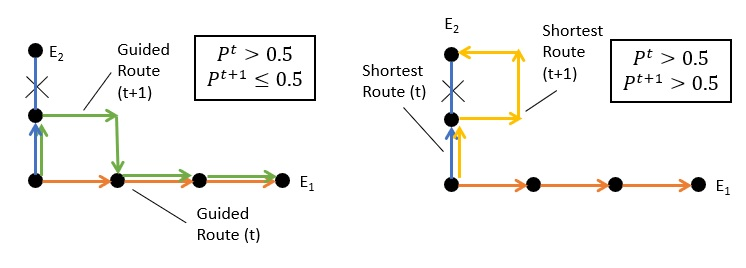
\includegraphics[width=15cm]{123.jpg}
\caption{Two Cases of the Route Taken by the "Selfish" Person}
\label{fig4-2}
\end{figure}

$P^{t}_x$ can be forecasted since we can observe the behavior of the person in last periods. Below we illustrate how to forecast $P^{t}_x$ by utilizing the \textbf{exponential smoothing method}.
\begin{equation}
\label{equ6}
For\ x\in  \bm{M}, \ \ 
P^{t+1}_x=\eta \gamma ^t_x+(1-\eta )P^t_x
\end{equation}
where $\bm{M}$ is the set of all the persons in the building, $\eta$ represents the smoothing coefficient, and $\gamma ^t_x$ follows:
\begin{equation}
\label{equ7}
\gamma^t_x=\left\{\begin{matrix}
1 & x\ doesn't\ follow\ the\ guide\\ 
0 & x\ follow\ the\ guide
\end{matrix}\right.
\end{equation}

Rearranging (\ref{equ6}) produces
\begin{equation}
\label{equ8}
    P^{t+1}_x=\eta \gamma ^t_x +(1-\eta)*\eta \gamma^{t-1}_x + \ldots + (1-\eta)^i \eta \gamma^{t-i}_x+ \ldots + (1-\eta)^t P^1_x
\end{equation}

Here we assume $\eta=0.8$, so we can get
\begin{equation}
\label{equ9}
P^{t+1}_x=0.8\gamma ^t_x+0.16\gamma ^{t-1}_x+0.032\gamma ^{t-2}_x + \ldots
\end{equation}

It implies that the "older" the observation value is, the smaller effect it has on the forecast of the possibility.

\subsection{Disabled People \& Emergency Personnel: Adjusted GUSH Model}
To take the disabled people and the emergency Personnel into consideration, we add a disabled people factor and emergency personnel factor into our GUSH model:
\begin{equation}
\label{equ10}
    C^t_{ij}=C^{t-1}_{ij}-s^{t-1}_{ij}-d^{t-1}_{ij}-e^{t-1}_{ij},\quad t=2,3,\ldots,n
\end{equation}

Similar to the selfishness factor, we have
\begin{equation}  
\label{equ11}
a^{t+1}_{xij}=
\left\{
  \begin{array}{ll}
    1 & v_i v_j\in \bm{F}^{t+1}_x\\ 
    -1 & v_i v_j\in \bm{C}^{t+1}_x\\ 
    0 & else
  \end{array}
\right.
\end{equation}
\begin{equation}
\label{equ12}
d^{t+1}_{ij}=\sum_{x=1}^{\left | \bm{D}  \right |} a^{t+1}_{xij}  
\end{equation}
where $\bm{F}^{t+1}_x$ is set of the edges the disabled person/emergency personnel person x take at the time period $t+1$, $\bm{C}^{t+1}_x$ is the set of the edges of the guided route the disabled person/emergency personnel person x should take initially, $d^1_{ij}=0$.

For the emergency personnel, they should take the shortest way to the bottlenecks. For the disabled, they should take the shortest way to the elevators specially prepared for them. We use the Dijkstra Algorithm to formulate the shortest route. However, the disabled people can't take the passage that's too crowded out of safety. We use $g^t_{ij}$ to indicate the population density of the edge $ij$ in the time period $t$.
\begin{equation}
\label{equ13}
    g^t_{ij}=f^t_{ij}/c^t_{ij}
\end{equation}

We assume the disabled can only take the passages whose population density are no more than 0.5. Below we show the set of the passages acceptable for them.
\begin{equation}
\label{equ14}
    \bm{G}^t=\{v_iv_j|g^t_{ij}>0.5\}
\end{equation}
\begin{equation}
\label{equ16}
    \bm{D}^{t+1}_x=\{v_iv_j|v_iv_j\notin \bm{G}^t\}
\end{equation}

In conclusion, \textbf{the adjusted GUSH model is presented as follows.}
\begin{eqnarray}
\label{equ18}
 & \textrm{maximize} &               \ \ 
 \sum \limits_{(v_i,v_j)\in \bm{E}} f^t_{ij},\quad t=1, 2, \ldots,n
 \nonumber
 \\
 & \textrm{subject}\ \textrm{to} &    \ \ 
\sum_{(v_i,v_k) \in  \bm{E}}f^t_{ik} - \sum_{(v_j,v_i)\in  \bm{E}}f^t_{ji}= 
\left\{\begin{matrix}
\sum\limits_{(v_i,v_j) \in  \bm{E}}f^t_{ij} & i=s\\ 
0 & i \neq s,e\\ 
-\sum\limits_{(v_i,v_j) \in  \bm{E}}f^t_{ij} & i=e
\end{matrix}\right.
\\
 &   &  \ \  
 0\leq f^t_{ij}\leq C^t_{ij} \nonumber
 \\
 &  & \ \ 
 C^t_{ij}=C^{t-1}_{ij}-s^{t-1}_{ij}-d^{t-1}_{ij}-e^{t-1}_{ij} \nonumber
\end{eqnarray}
where $v_i$ denotes the node $i$,  $f^t_{ij}$ and $C^t_{ij}$ respectively represent the flow and the capacity of the edge $v_iv_j$ in the time period $t$, $s^{t}_{ij}$ is defined in (\ref{equ3}) and (\ref{equ4}), $d^{t-1}_{ij}$ and $e^{t-1}_{ij}$ are defined in (\ref{equ12}) and (\ref{equ13}).

\section{Model Applying to the Louvre}
\subsection{Basic Network Model in the Ideal Situation}
\paragraph{Drawing the network graph} According to the tourist map, we draw the network graph of each floor of the museum. The graph of Floor 0 and -1 are shown as follows.

\begin{figure} [H]
\centering
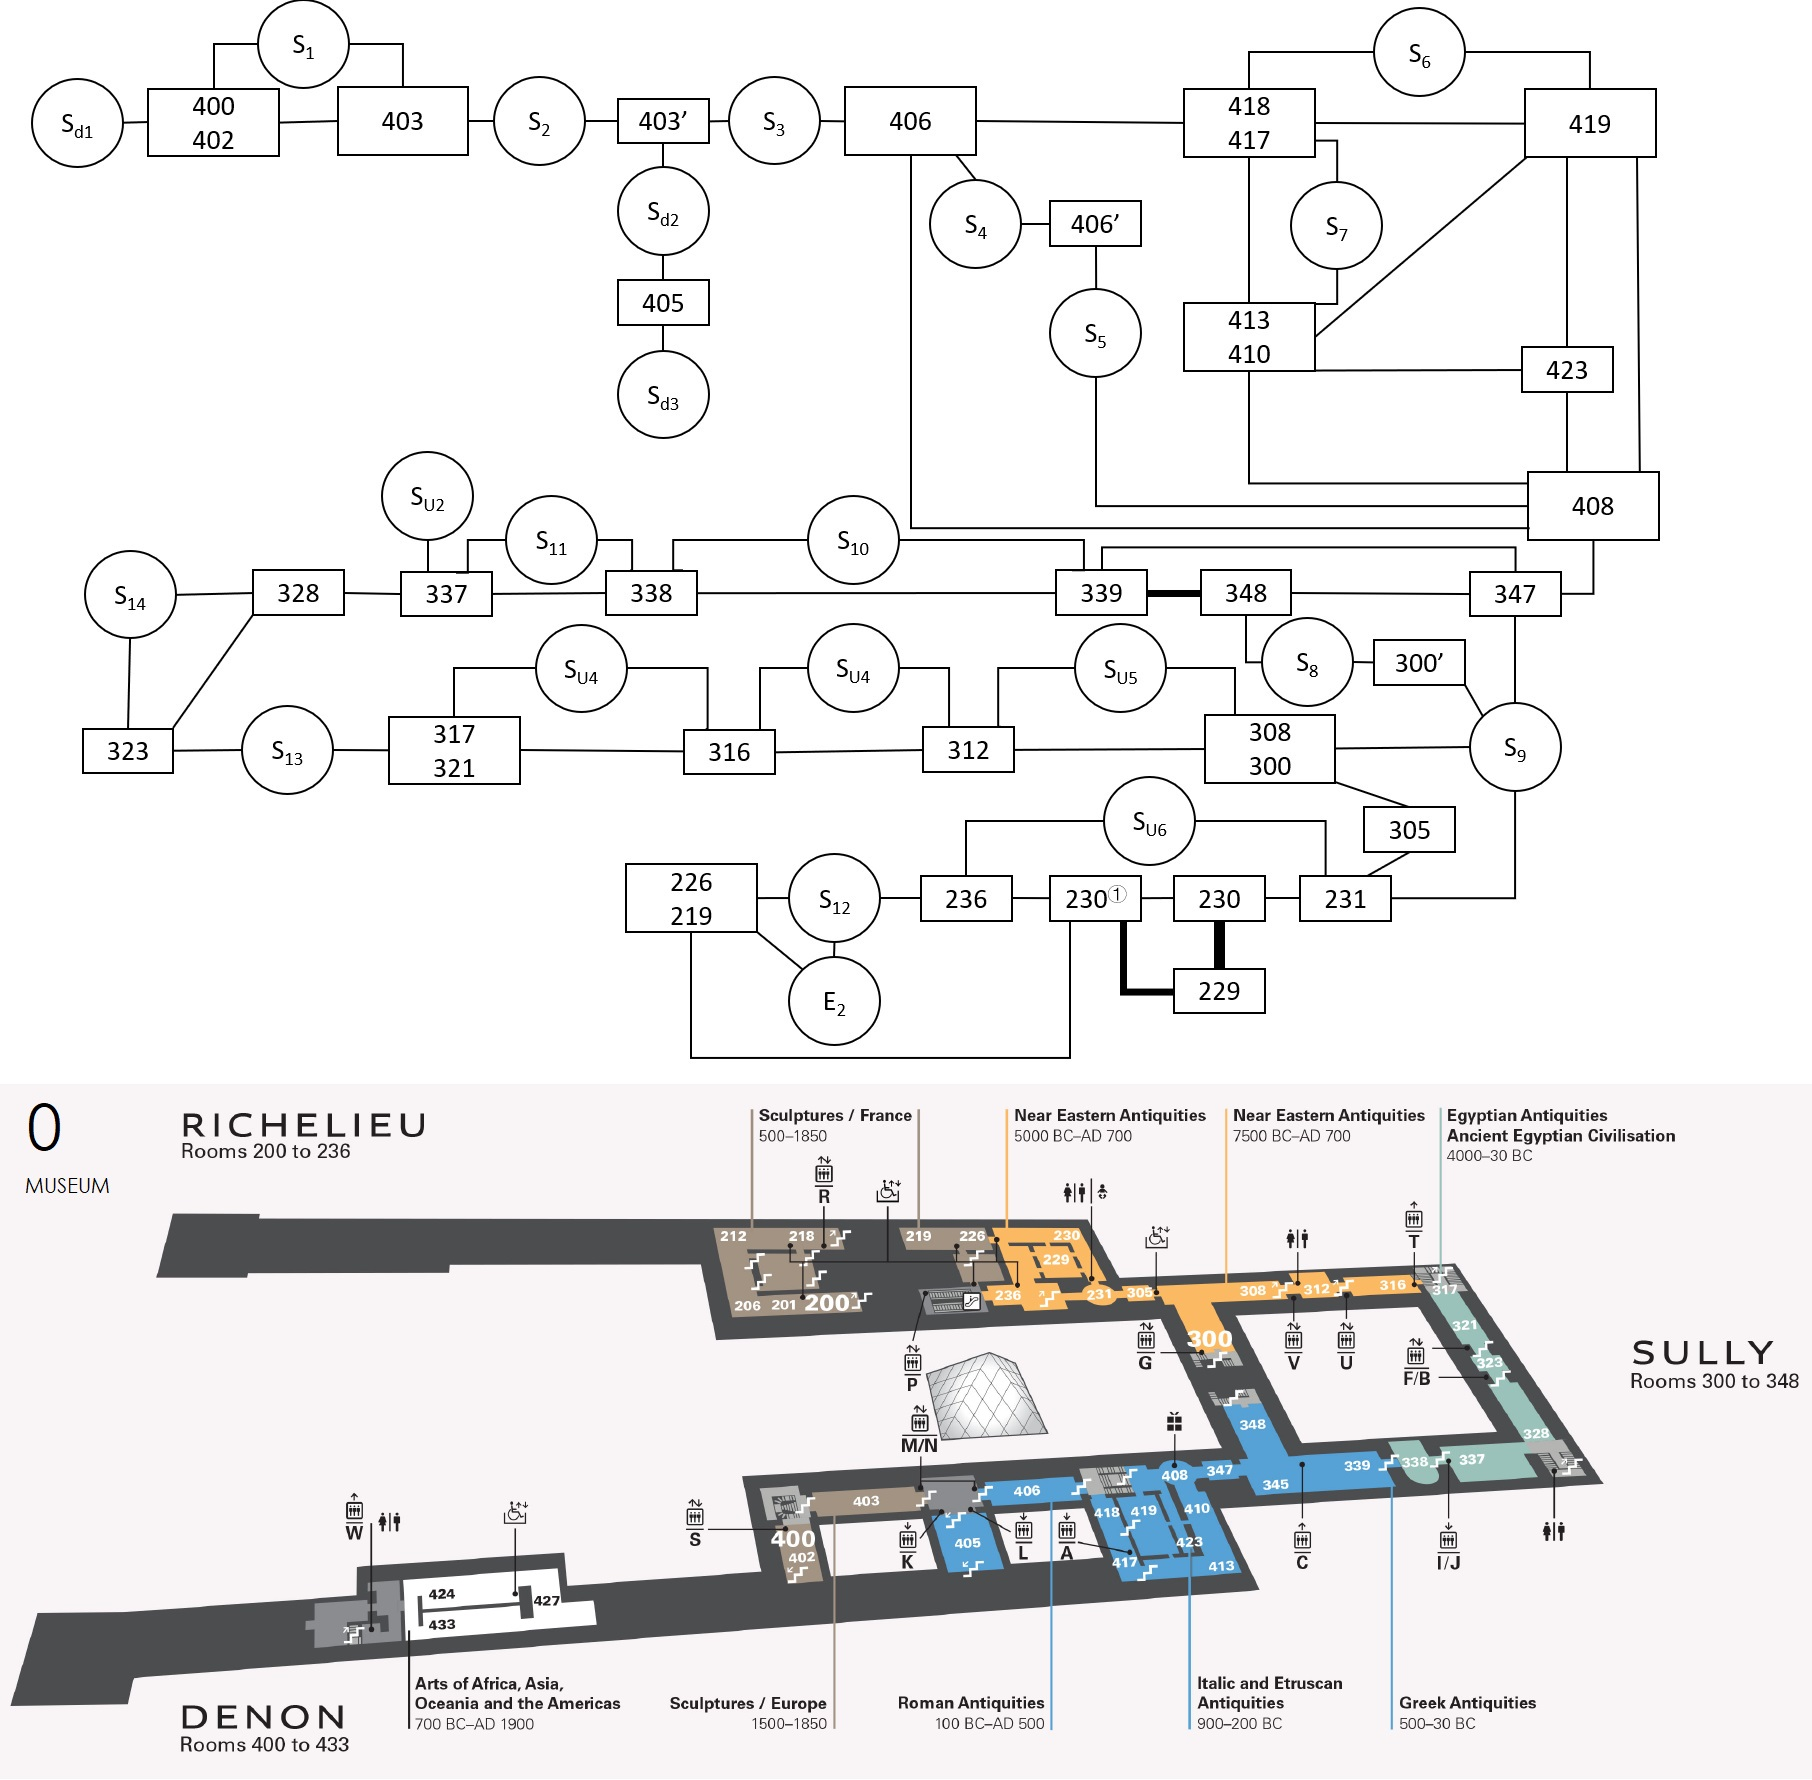
\includegraphics[width=15cm]{floor_0_comp.jpg}
\caption{Network Graph of the Floor 0}
\label{fig5-1}
\end{figure}

\begin{figure} [H]
\centering
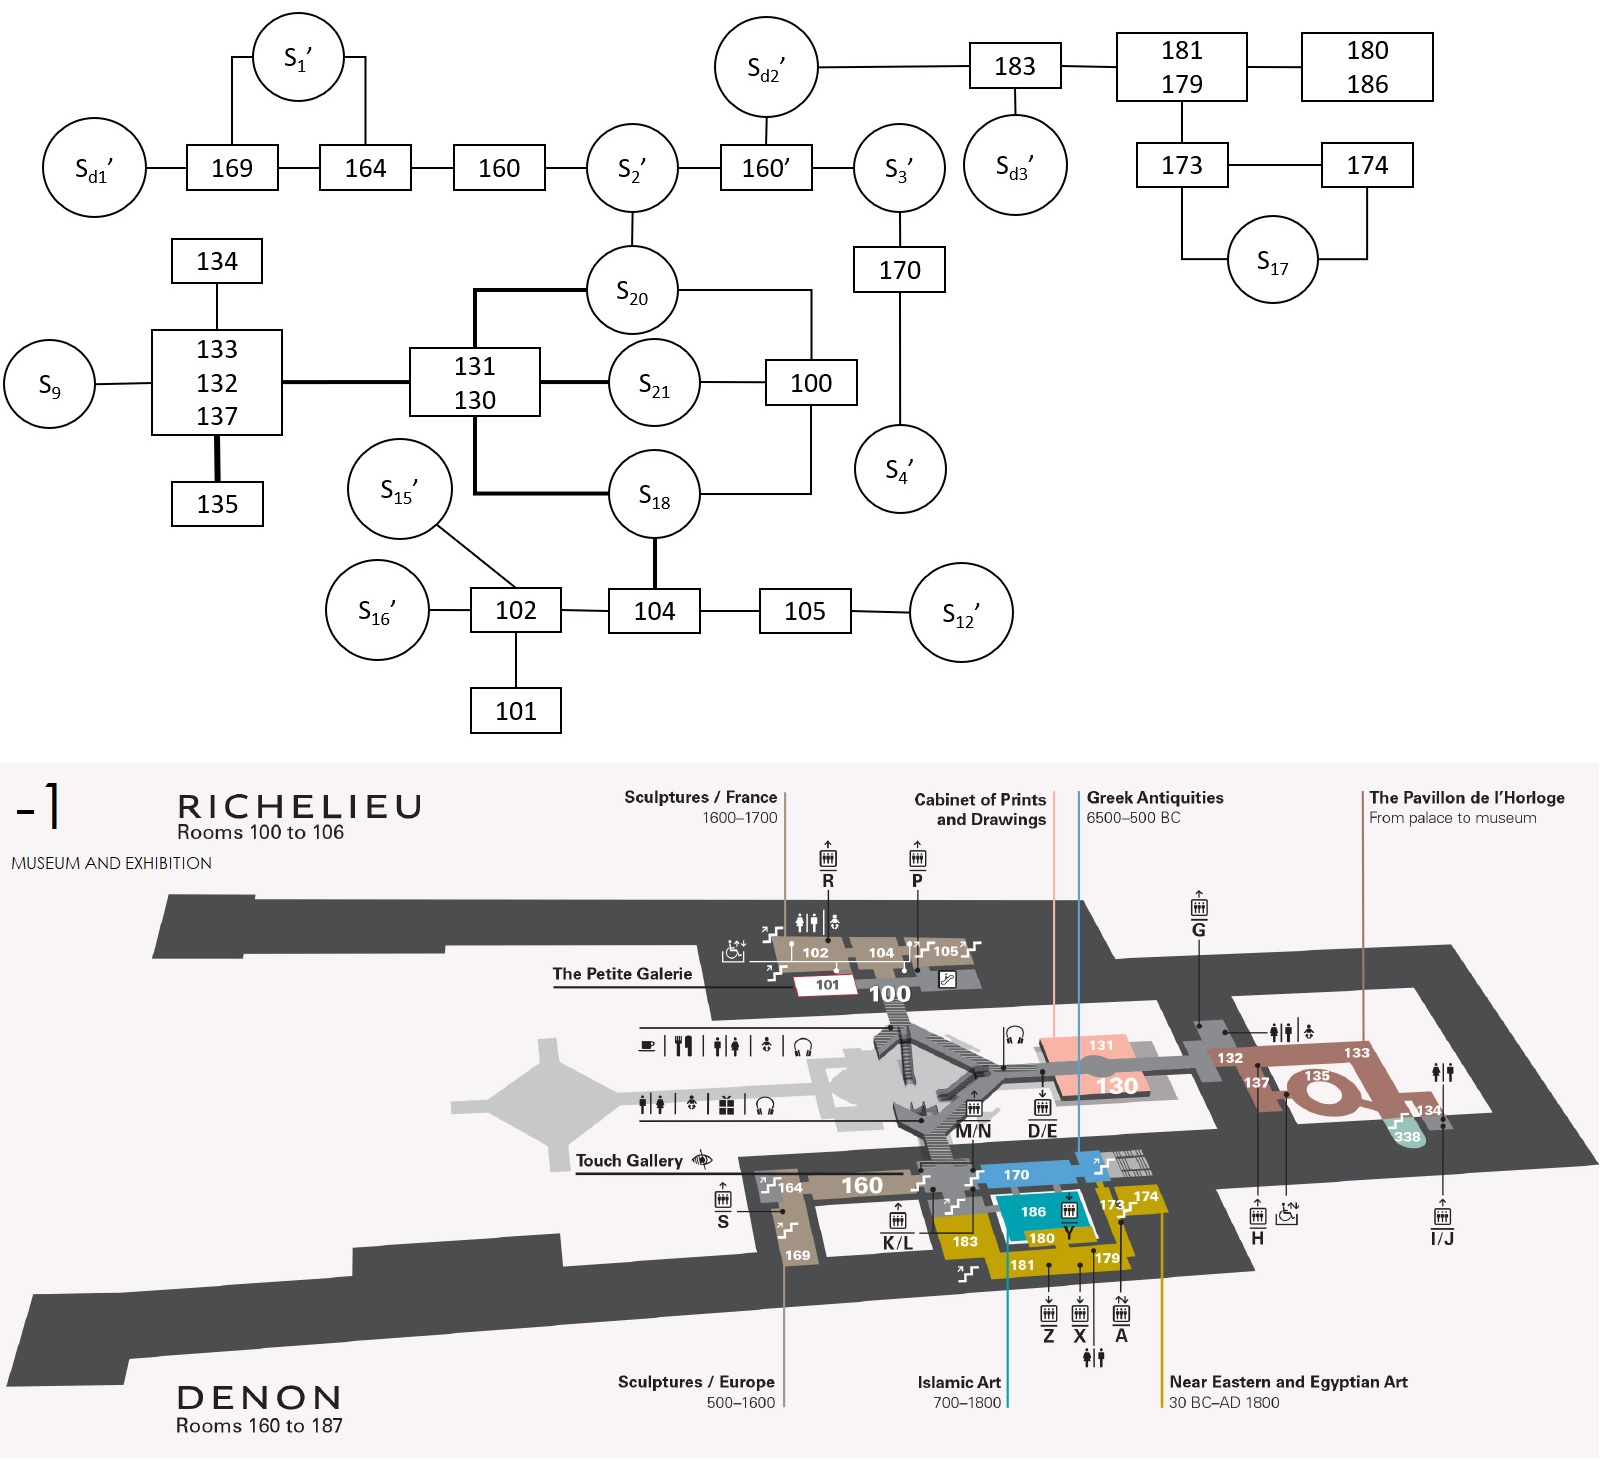
\includegraphics[width=15cm]{floor_u1_comp.jpg}
\caption{Network Graph of the Floor -1}
\label{fig5-2}
\end{figure}

In Figure \ref{fig5-1} and Figure \ref{fig5-2}, the nodes are stylized as to suggest different building components, among which squares represent rooms, with the label of each room inside, circles represent stairs and lines represent passages, whose degree of thickness indicates the capacity. On each floor there are three kinds of stairs: the stairs only for walking up (which is represented by $S_u$), only for walking down ($S_d$) and for both up and down ($S$).

By determining the scale, we get the space area of rooms, passages and stairs. We use these data to estimate the capacity, assuming that the capacity is proportional to the space area. 
\paragraph{Calculating the network model} We adopt the 
the procedure of Edmond-Karp algorithm to run this dynamic maximal flow model. In this ideal situation, where everyone follows the App, it takes 11.6 minutes for all the occupants to go out. Figure \ref{fig5-3} shows the population density of one period during the whole evacuation periods.

\begin{figure} [H]
\centering
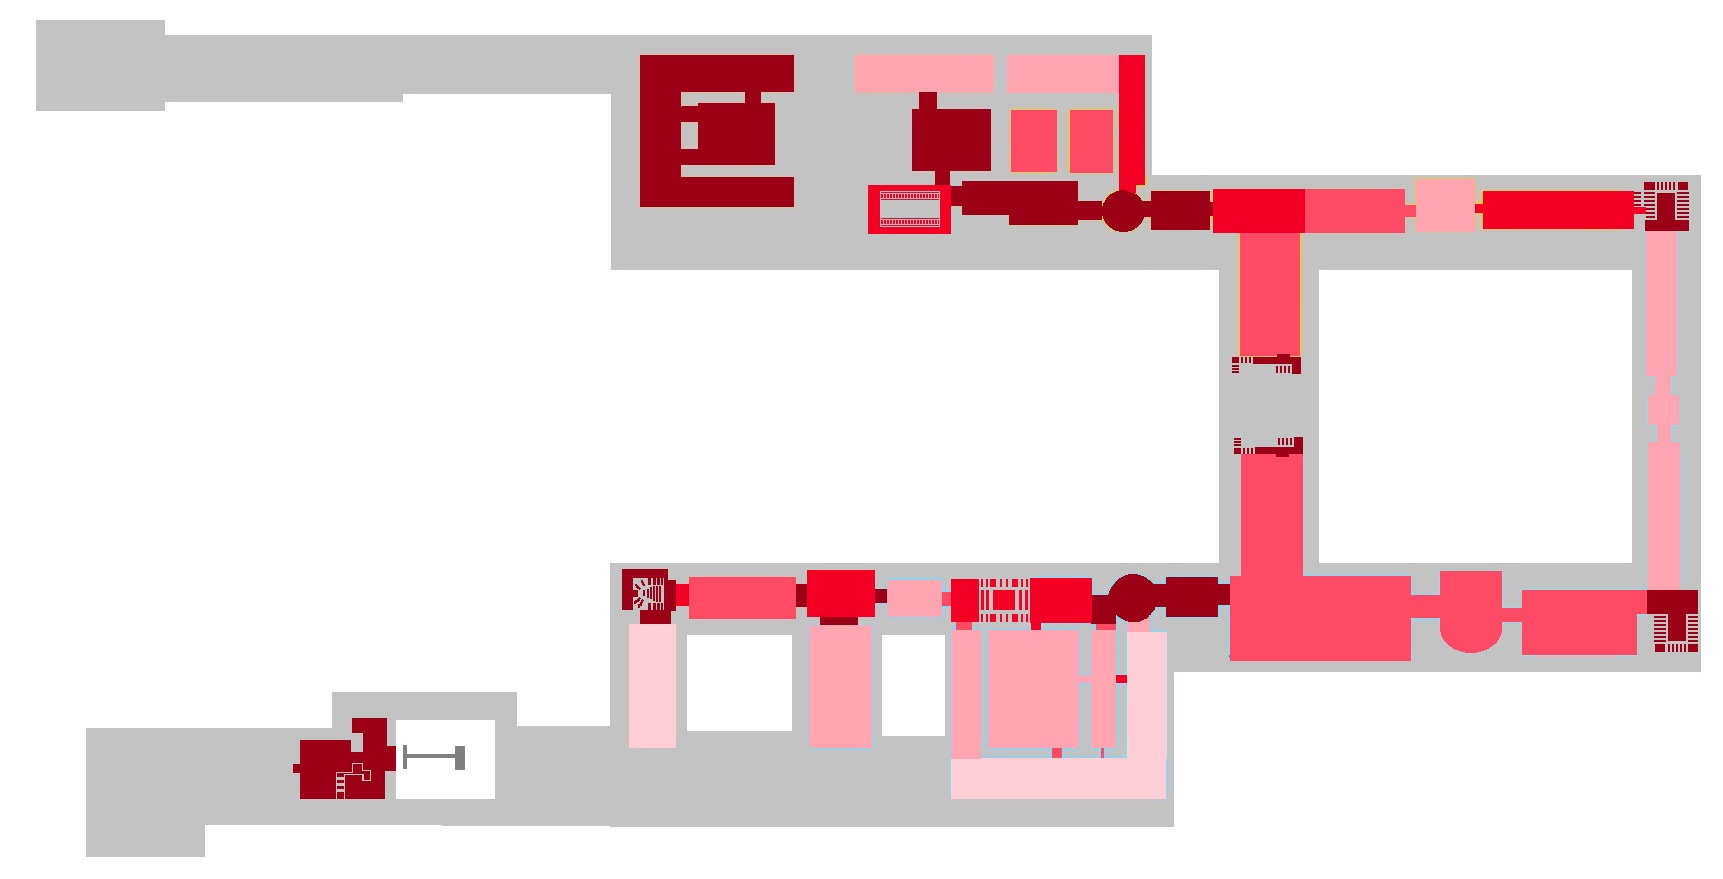
\includegraphics[width=15cm]{1234.jpg}
\caption{Population Density Graph of the Maximal Flow Model (the darker the colour, the denser the population)}
\label{fig5-3}
\end{figure}
According to the computer run of the model, there are altogether 38 bottle necks. Most are the stairs and passages directly connected to the exit. Some passageways between rooms that are slim are also bottle necks, such as Room 408 to Room 347, Room 183 to Room 181.

\subsection{GUSH Model Considering Specific Problems}
We calculate the GUSH model. Based on the results, the evacuation time is 15.2 minutes and the number of bottlenecks is 45. Figure \ref{fig5-4} shows the population density of one period during the whole evacuation periods.
\begin{figure} [H]
\centering
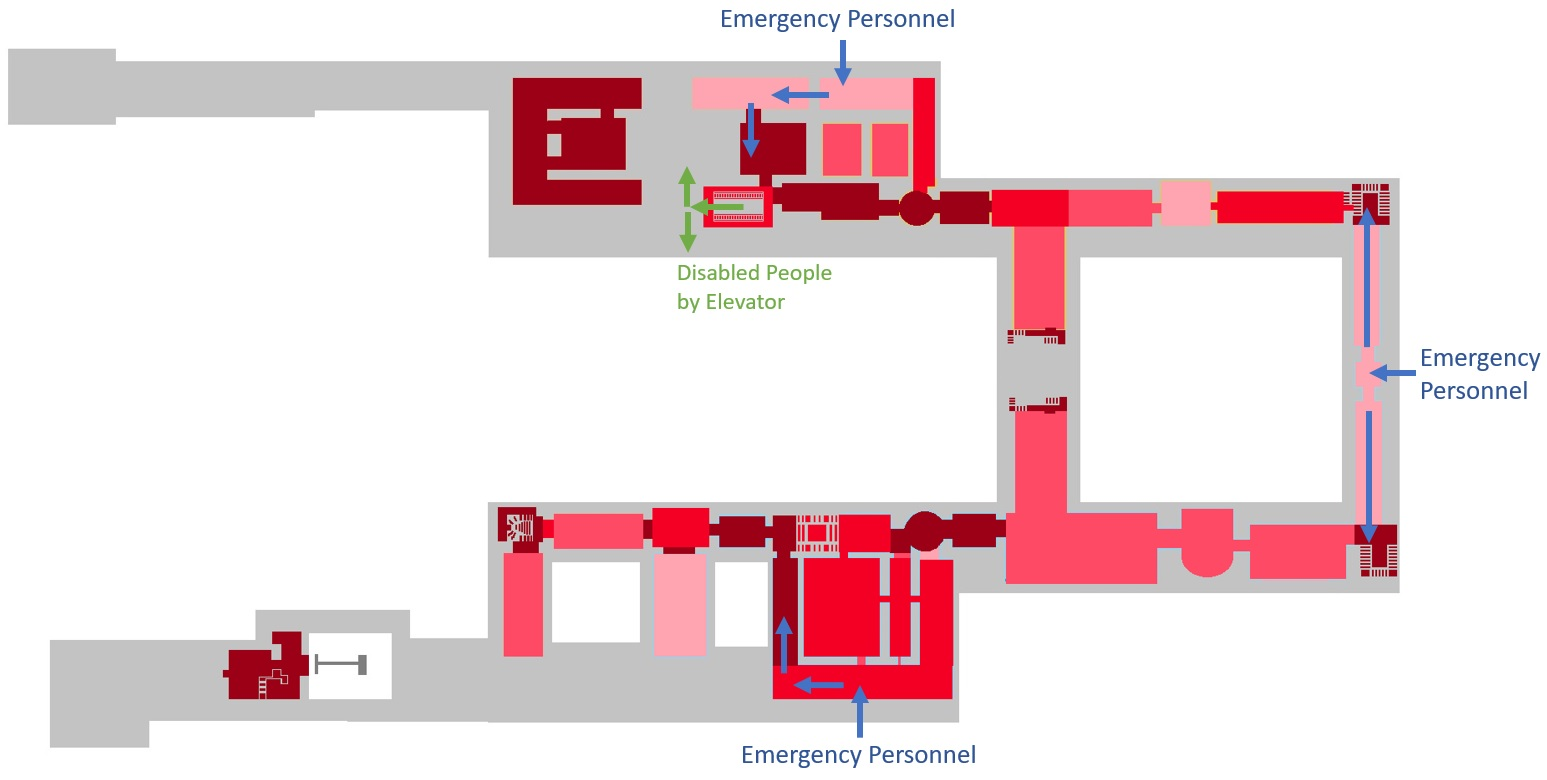
\includegraphics[width=15cm]{ttest.jpg}
\caption{Population Density Graph of the Adjusted GUSH Model}
\label{fig5-4}
\end{figure}

As is shown in Figure \ref{fig5-4}, there are more bottlenecks than those in the ideal situation. For the route of the emergency personnel, we take three groups as an example. They enter the extra entrances and head for the bottlenecks via the shortest routes.
\subsection{An Example of Applying Our Model}
We create an example of terror attack in the Louvre to justify our model. Assuming that on December 29th, 2019, a terror attack happens in the Room 338 on the ground floor. The managers use the GUSH model to give guidance for everyone. Figure \ref{fig5-5} shows the changed network flow graph according to the reality. 

\begin{figure} [H]
\centering
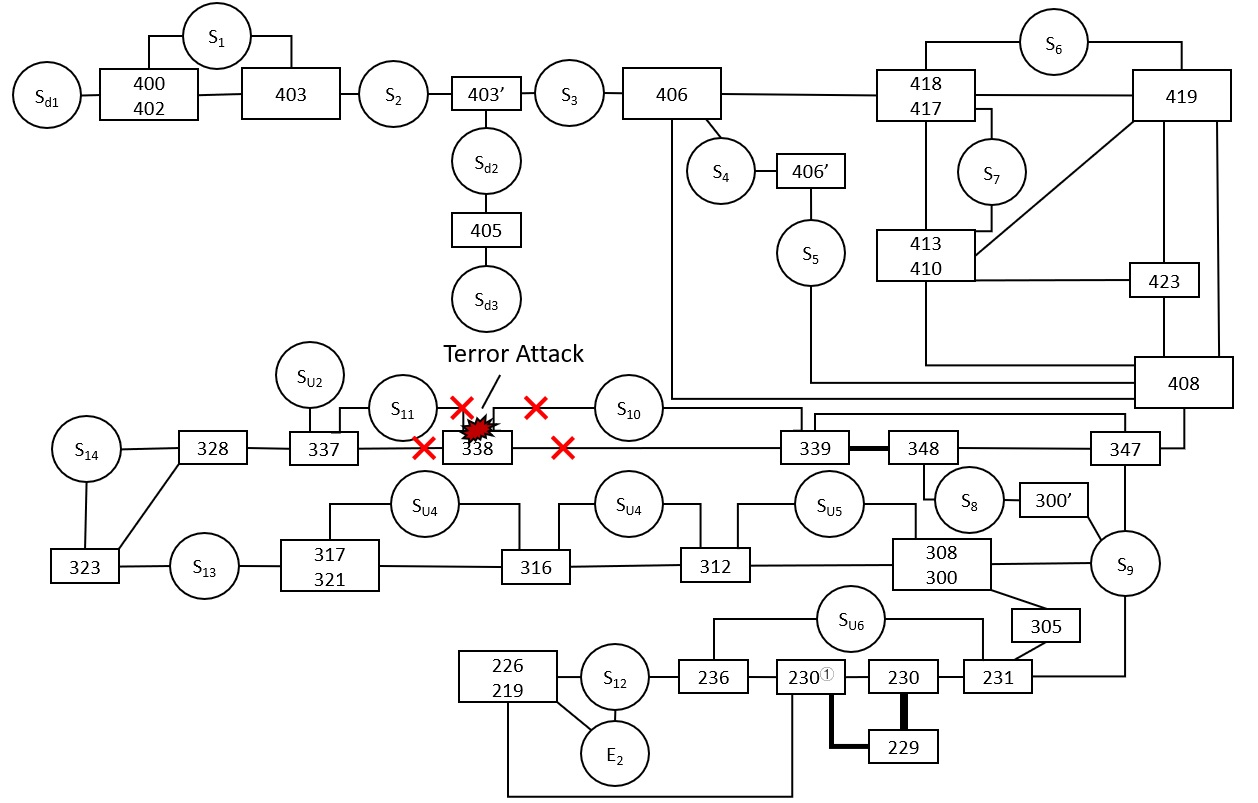
\includegraphics[width=15cm]{floor_0_new_new.jpg}
\caption{Changed Network Flow Graph in the Case of Terror Attack}
\label{fig5-5}
\end{figure}

From Figure \ref{fig5-5}, we can see that the edges connecting the room where terror attack happens are removed. Calculating the model, we get the evacuation time, 18.3 minutes and the bottleneck, 48. Figure \ref{fig5-6} shows the population density of one period during the whole evacuation periods.
\begin{figure} [H]
\centering
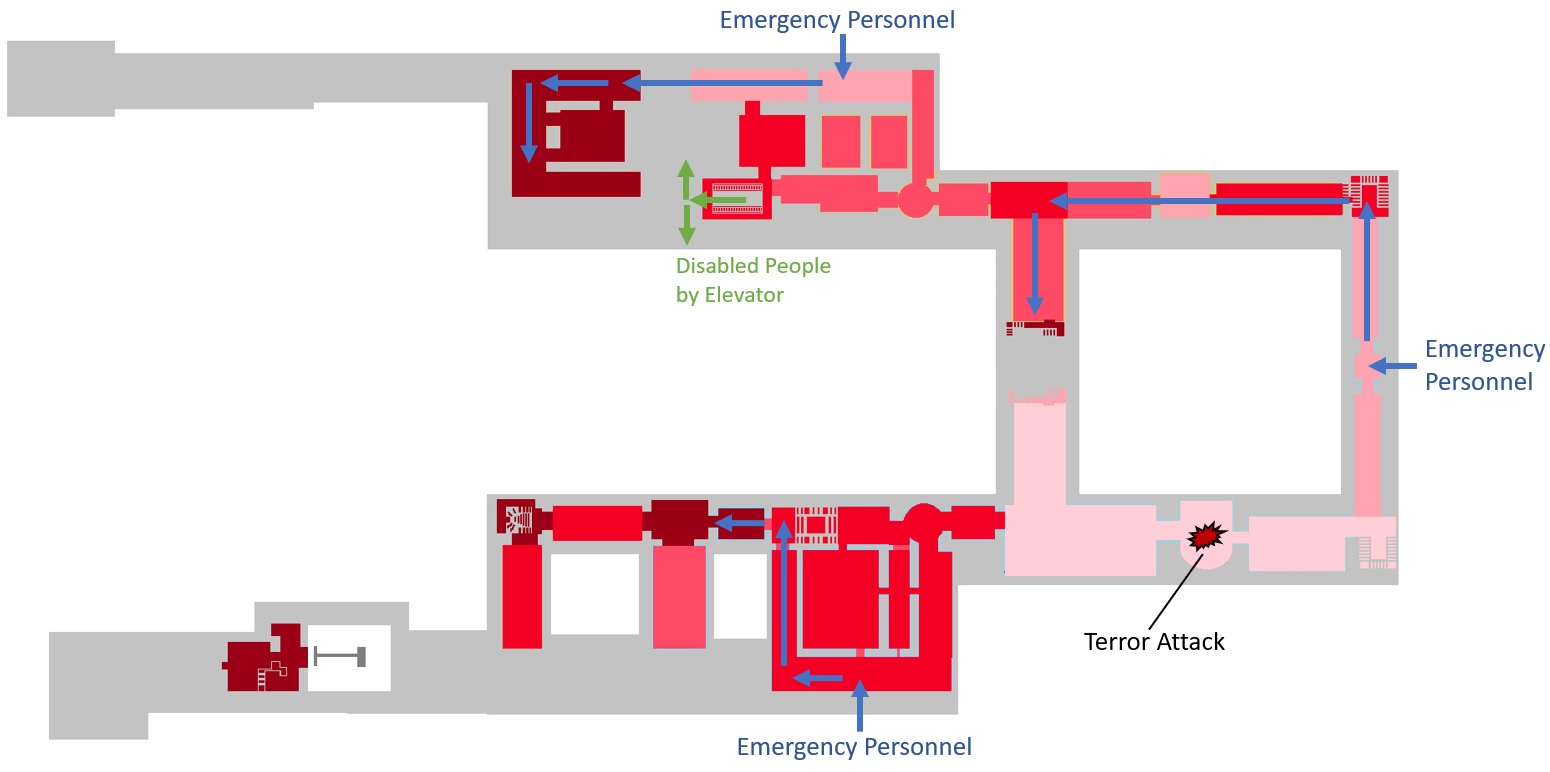
\includegraphics[width=15cm]{app3.jpg}
\caption{Population Density Graph in the Case of Terror Attack}
\label{fig5-6}
\end{figure}
As is shown in Figure \ref{fig5-6}, the evacuation plan changes. The route of the emergency personnel also changes. This implies that our model is adaptable enough to react quickly to different emergencies.

\section{Sensitivity Analysis}
In this section, we change the value of the two parameters, the length of each time period and the capacity of the bottlenecks, in our adjusted GUSH model and test their influence on the evacuation time. 
\subsection{Faster is Slower}
In our model, time is divided into time periods which are very short and of equal length so that we can recalculate results in every time period to provide real-time evacuation plans. The time period length is determined in consideration of the crowd flow rate. For example, if people run fast, we should shorten the time period length to update paths more frequently, and vice versa. Thus, the change of the time period length may well affects the outcome. 

When applying our model in the above case, the time period length is set as 5 seconds under the assumption that people move at the speed of 1m/s. When people move faster or slower a bit, the time period length have many different values. We test these values in our model and get the results as follows.
\begin{table}[ht]
  \caption{Evacuation Time Change with the Time Period Length}
  \label{tab3}
  \centering
  \begin{threeparttable}
    \setlength{\extrarowheight}{2mm}
    \begin{tabular}{|c|ccccccccccc|}
    \hline
    \rowcolor[gray]{0.9}
    TPL\tnote{1}&3    & 3.3  & 3.6  & 3.9  & 4.2  & 4.5  & 4.8  & 5.1  & 5.4 & 5.7  & 6.0 \\
    \rowcolor{mycyan}
    ET \tnote{2}&20.9 & 19.8 & 18.6 & 17.6 & 16.8 & 16.2 & 15.6 & 15.3 & 16.3& 18.6 & 2.7\\
    \hline
    \end{tabular}
        \begin{tablenotes}
        \footnotesize
        \item[1] Time Period Length
        \item[2] Evacuation Time
      \end{tablenotes}
          \end{threeparttable}
\end{table}

\begin{figure} [H]
\centering
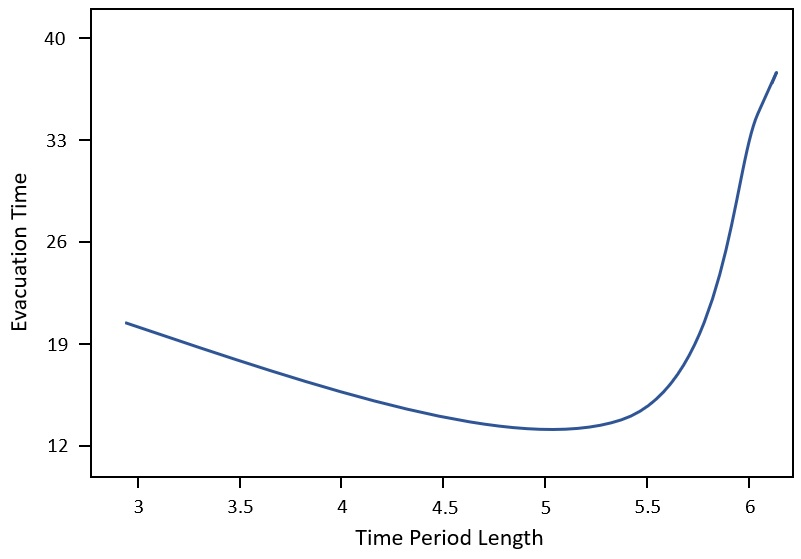
\includegraphics[width=10cm]{time_period.jpg}
\caption{Evacuation Time Change with the Time Period Length}
\label{fig8}
\end{figure}

As is shown in Figure \ref{fig8}, with the time period length increasing from 3s to 6s at the step of 0.2s, the evacuation time takes on an "U" shape, i.e., it reduces first and then increases. As mentioned above, the time period length reflects the crowed flow rate. The smaller length value indicates the larger flow rate. Thus, Figure \ref{fig8} can be also interpreted as a relationship between the crowed flow rate and the evacuation time, which is still an "U" shape, i.e., the slow or fast enough crowed flow rate leads to a long evacuation time.

From the analysis above, we find an interesting phenomenon: \textbf{faster is slower}. That is to say, if everyone seeks to reach a high moving speed, instead of being faster, the crowd flow rate for all slow down, eventually causing block.

\subsection{Optimal Expansion Percentage of Bottlenecks}

According to the application of our model in the above case, 45 bottlenecks are examined out of nearly 300 passages. Hence, we can recommend the managers to expand the capacity of some bottlenecks to reduce the possibility of block. However, the specific expansion percentage can be difficult to determine, because more expansion will inevitably lead to higher costs.

To figure out the expansion problem, we test the edge capacity parameter in our model to simulate the process of expansion, while observing the change of the evacuation time. For all the bottleneck edges, we increase part of their capacity values and get the results as follows.

\begin{table}[ht]
  \caption{Evacuation Time Change with the Expansion Percentage of Bottlenecks}
  \label{tab2}
  \centering
  \begin{threeparttable}
    \setlength{\extrarowheight}{2mm}
    \begin{tabular}{|c|ccccccccccc|}
    \hline
    \rowcolor[gray]{0.9}
    EPB\tnote{1} &0       & 0.1   & 0.2  & 0.3  & 0.4  & 0.5  & 0.6  & 0.7  & 0.8 &0.9    &1\\
    \rowcolor{mycyan}
    ET\tnote{2} &15.2    &14.6   & 12.9 & 11.2 & 8 & 7.8 & 7 & 6.9 & 6.8 & 6.7 & 6.7\\
    \hline
    \end{tabular}
        \begin{tablenotes}
        \footnotesize
        \item[1] Expansion Percentage of Bottlenecks
        \item[2] Evacuation Time
      \end{tablenotes}
          \end{threeparttable}
\end{table}

\begin{figure} [H]
\centering
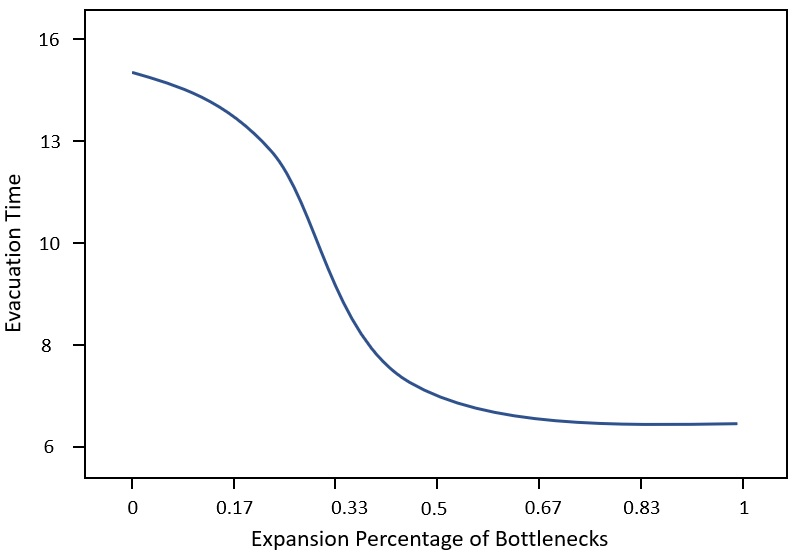
\includegraphics[width=10cm]{expansion.jpg}
\caption{Evacuation Time Change with the Expansion Percentage of Bottlenecks}
\label{fig9}
\end{figure}
As is shown in Figure \ref{fig9}, we adjust the values of expansion percentage of bottlenecks in the interval of [0,1], with 0 representing no expansion at all and 1 representing doubling the original capacity. The evacuation time changes accordingly. With the expansion of the bottlenecks, the speed at which the evacuation time gets shorter tends to slow down.

Observing the trend, we can draw a conclusion: \textbf{the optimal expansion percentage of bottlenecks is around 60\%}. Because when the percentage exceeds this threshold, the declining rate of evacuation time approaches zero. In other words, in this period, expanding bottlenecks is worthless, for it will not bring about any change in evacuation time basically.

\section{Strengths and Weaknesses}
\subsection{Strengths}
\paragraph{Viewing from different angels} We develop our model from two angles. One is in the manager's position, the other is from the view of the evacuees. Thus our model is creative and considerable.
\paragraph{Considering different groups} We take different groups into consideration, including selfish people, disabled people and emergency personnel, making our model
comprehensive and and reflect the reality well.
\subsection{Weaknesses}
\paragraph{Demanding certain technology} In our model, the plan is dynamic and real-time, depending on the location of people. So we require that the managers of the museum can locate everyone and provide guide function in the official App.
\paragraph{Lacking accurate information} Because of several factors not considered and the lack of data, our model are not enough to indicate the accurate situation which has a risk of error.
\section{Conclusions}
In this paper, we develop a GUSH model to help the managers of the Louvre make an evacuation plan, which contains:
\begin{itemize}
\item An optimal route for each employee, including the special route for the disabled people. 
\item An optimal route for the emergency personnel entering the museum and the way of using the extra entrances.
\item A global population distribution graph, showing the bottlenecks, which are critical for the managers to do the crowd control.
\end{itemize}

Based on our analysis, we propose several recommendations for the emergency management of the Louvre:
\begin{itemize}
\item The museum can add the evacuation guide function in their official App. The App is extremely efficient in planning the optimal route consuming the shortest time in a global view.
\item To improve the evacuation efficiency, the museum can do some reconstruction. According to our sensitivity analysis, the best strategy is to increase 60\% of the capacity of the bottlenecks, which can shorten the evacuation time to a high degree. 
\end{itemize}

By adopting our GUSH model and making the most of technology, the museum emergency management can react quickly to any emergency. The GUSH model is also adaptable. It can be adopted to help design the evacuation plan for other large, crowded structures.
\addcontentsline{toc}{section}{Reference}
\bibliographystyle{apalike}
\bibliography{icmmcm}




\end{document}


